\title{Podkmen: Obratlovci}
\documentclass[10pt,a4paper]{article}
\usepackage[utf8]{inputenc}
\usepackage[czech]{babel}
\usepackage{amsmath}
\usepackage{amsfonts}
\usepackage{amssymb}
\usepackage{chemfig}
\usepackage{geometry}
\usepackage{wrapfig}
\usepackage{graphicx}
\usepackage{floatflt}
\usepackage{hyperref}
\usepackage{fancyhdr}
\usepackage{tabularx}
\usepackage{makecell}
\usepackage{csquotes}
\usepackage{footnote}
\usepackage{movie15}
\MakeOuterQuote{"}

\renewcommand{\labelitemii}{$\circ$}
\renewcommand{\labelitemiii}{--}
\newcommand{\ra}{$\rightarrow$ }
\newcommand{\x}{$\times$ }
\newcommand{\lp}[2]{#1 -- #2}
\newcommand{\timeline}{\input{timeline}}


\geometry{lmargin = 0.8in, rmargin = 0.8in, tmargin = 0.8in, bmargin = 0.8in}
\date{\today}
\author{Jakub Rádl}

\makeatletter
\let\thetitle\@title
\let\theauthor\@author
\makeatother

\hypersetup{
colorlinks=true,
linkcolor=black,
urlcolor=cyan,
}



\begin{document}
\maketitle
\tableofcontents
\begin{figure}[b]
Toto dílo \textit{\thetitle} podléhá licenci Creative Commons \href{https://creativecommons.org/licenses/by-nc/4.0/}{CC BY-NC 4.0}.\\ (creativecommons.org/licenses/by-nc/4.0/)
\end{figure}
\newpage

\section{Úvod}
\subsection{Základní charakteristika obratlovců}
Živočichové $>$ Triblastica $>$ Druhoústí $>$ Strunatci $>$ Obratlovci
\begin{itemize}
\item nejpočetnější podkmen strunatců
\item \textbf{aktivně pohybliví}, bilaterálně souměrní
	\begin{itemize}
	\item příčně pruhovaná, hladká, srdeční svalovina
	\end{itemize}
\item mimořádně výkonná NS a smyslové orgány
\item tělo členěno na \textbf{hlavu, trup a ocas}
\item \textbf{pokožka} vždy \textbf{vícevrstevná}, produkuje různé deriváty (šupiny, peří, srst, \ldots)
\item struna hřbetní potlačena u dospělých jedinců a nahrazena vnitřní koštěnou kostrou s malým podílem chrupavek
\item končetiny mají jednotný stavební plán, mají koštěnou vnitřní stavbu
\end{itemize}

\subsection{Systém}
\begin{tabular}{|c|c|c|c|c|c|c|c|}
\hline
Třídy&kruhoústí&paryby&ryby&obojživelníci&plazi&ptáci&savci		\\ \hline
Přítomnost čelistí&bezčelistnatci& \multicolumn{5}{c}{čelistnatci} &		\\ \hline
Prostředí, kde žijí & \multicolumn{2}{c}{ploutvovci (Pisces)} && \multicolumn{3}{c}{čtyřnožci (Tetrapoda)} &\\ \hline
Prostředí vývoje vajec & \multicolumn{3}{c}{bezblanní (Anamnia)} && \multicolumn{2}{c}{blanatí(Amniota)} &		\\ \hline
\makecell{Schopnost udržovat \\ stálou tělesnou teplotu}	& \multicolumn{4}{c}{ektotermní} && \multicolumn{1}{c}{endotermní} &	\\ \hline
\end{tabular}

\paragraph{Přítomnost čelistí}
\begin{itemize}
\item čelisti vytvořeny z prvního páru žaber
\item bezčelistnatí mají 7 párů žaber
\end{itemize}

\paragraph{Prostředí}
\begin{itemize}
\item podobnosti ve stavbě ploutví a nohou
\end{itemize}

\paragraph{Prostředí vývoje vajec}
\begin{itemize}
\item bezblanní(\textit{Anamnia}) se rozmnožují ve vodě
\item blanatí (\textit{Amniota}) má vnitřní vodní prostředí \ra mohou se rozmnožovat na souši
\end{itemize}

\paragraph{Udržování teploty}
\begin{itemize}
\item studenokrevní (ektotermní)
\item teplokrevní (endotermní) -- velká spotřeba energie
\end{itemize}

\newpage
\section{Nadtřída: Bezčelistnatci}
\begin{itemize}
\item 7 párů žaber
\item hadovitý tvar těla
\item produkce slizu -- snižuje riziko uchopení predátorem
\end{itemize}

\subsection{Třída: Kruhoústí}
\subsubsection{Podtřída: Sliznatky (\textit{Myxinoidea})}
\begin{itemize}
\item obývají mořské dno
\item destruenti -- vyžírají orgány z mrtvých / velmi zraněných ryb
\end{itemize}

\subsubsection{Podtřída: Mihule (\textit{Petromyzontida})}
\begin{itemize}
\item larva \textbf{minoha}
	\begin{itemize}
	\item pilovitý ústní disk \ra prořezávání ryb
	\end{itemize}
\item regresní vývoj (dospělec má zakrnělou trávící soustavu -> žije jen ze zásob a pak umře)
\end{itemize}

\paragraph{Mihule potoční, Mihule mořská}
\begin{itemize}
\item kriticky ohrožená
\end{itemize}

\newpage
\section{Nadtřída: Čelistnatci}
\subsection{Třída: Paryby}
\begin{itemize}
\item jednostranně orientované šupiny -- brání přisávání živočichů
\item vodní, převážně mořští
\item první objevení na konci prvohor a hlavní rozšíření v druhohorách
\end{itemize}

\paragraph{Tělo}
\begin{itemize}
\item velký rypec na přední straně
\item \textbf{Lorenziho ampule} (orgán) -- vnímá elektrické signály nervových soustav jiných živočichů
\end{itemize}

\subsubsection{Skupina: Chiméry}
\begin{itemize}
\item bizarně vypadající paryby
\item nepravá skřele -- krytka žáber
\end{itemize}

\subsubsection{Skupina: Příčnoústí}
\begin{itemize}
\item torpédovitý tvar
\item dlouhý rypec, ústa na spodní straně hlavy
\item struna zachována po celý život
\item první pár žaber přeměněn v čelisti, druhý pár v jazylku
\item \textbf{plakoidní šupiny}
\begin{itemize}
\item jediný výskyt kostní tkáně (tvořeny -- dentinem a emailem), zakotveny ve škáře
\end{itemize}
\end{itemize}

\paragraph{Kostra}
\begin{itemize}
\item široká lebka s pouzdry smyslových orgánů
\end{itemize}

\paragraph{Ploutve}\mbox{} \\ \mbox{} \\
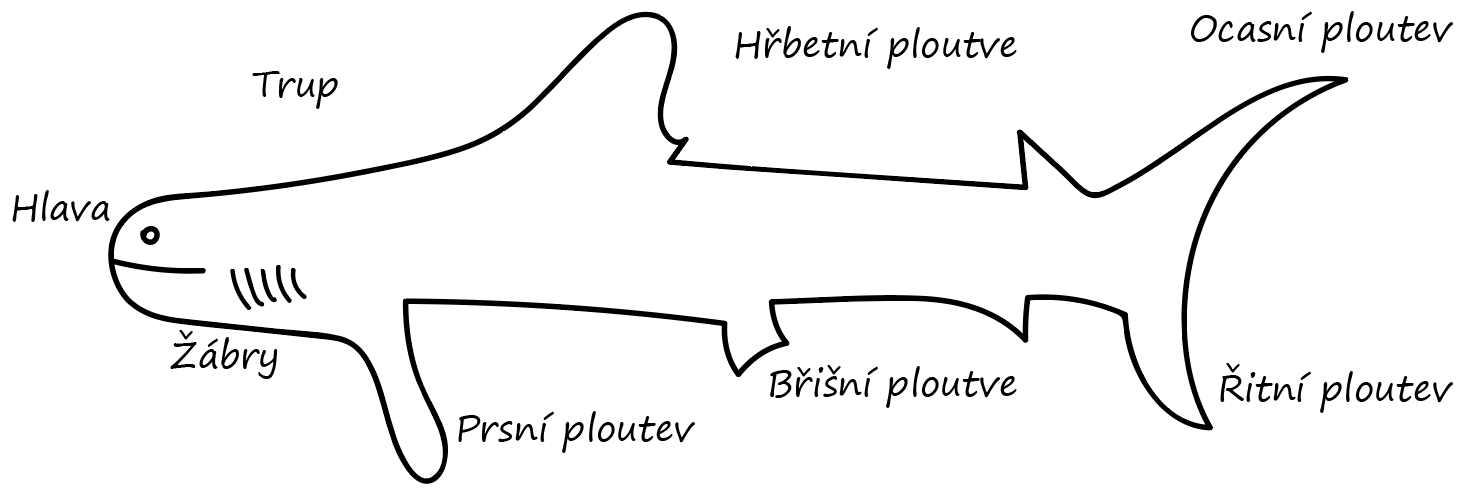
\includegraphics[width=\textwidth]{pictures/ploutve.png}


\paragraph{Nervová soustava}
\begin{itemize}
\item protáhlý mozek (už ne jen zauzlina)
	\begin{itemize}
	\item vyvinutý mozeček -- zodpovědný za koordinované pohyby
	\item čelní lalok -- čich
	\end{itemize}
\end{itemize}

\paragraph{Trávící soustava}
\begin{itemize}
\item ústa, zuby, hltan, jícen, žaludek, střevo
\item obrovská játra (10 - 20\% hmotnosti jedince) se žlučníkem 
\item hydrostatický orgán -- regulace hloubky ponoru
\item hypertonické prostředí \ra orgán na vylučování soli
\end{itemize}

\paragraph{Dýchací soustava} -- 2 páry žaber přeměněné na čelisti a jazylku, 5 párů zbylo

\paragraph{Cévní soustava} -- uzavřená, 1 předsíň, 1 komora, okysličení krve v žábrách

\paragraph{Rozmnožovací soustava}
\begin{itemize}
\item vnitřní oplození pomocí prsních ploutví
\item může se objevit živorodost (není placenta, ale žloutkový vak)
\item prenatální kanibalismus -- mláďata se mohou před narozením navzájem sníst
\end{itemize}


\paragraph{Ekologie}
\begin{itemize}
\item původně mořští, cca 30 sladkovodních druhů (15 smíšených)
\item podle druhu potravy dělíme na: lovce, plakntonofágy, bentofágy (rytí ve dně)
\end{itemize}

\paragraph{Chování} -- málo dlouhé, loví se k jídlu

\paragraph{Zástupci}
\begin{itemize}
\item \textbf{Žralok obrovský} -- planktonofágní
\item \textbf{Žralok bílý} -- 7m, 3.5t, nebezpečný pro člověka (živí se tvory u hladiny)
\item \textbf{Kladivoun obecný}
	\begin{itemize}
	\item oci na koncích hlavy
	\item velké množství Lorenziho ampulí na hlavě (elektrosensor)
	\end{itemize}
\item \textbf{Piloun mnohozubý} -- pentofág
\item \textbf{Trnucha obecná} -- u ocasu trn s jedovou žlázou, evropská pobřeží
\item \textbf{Manta atlanská} -- 9m 
\end{itemize}

\newpage
\section{Třída: Ryby}
\begin{itemize}
\item dle reálného členění by pod ryby spadal i člověk (pod plazy ptáci) \ra třída ryby reálně neexistuje

\end{itemize}


\end{document}